\section{Hardware}
\label{sec:hardware}

\subsection{Main interface board}

\subsubsection{Encoder}

On the motor is an \textit{AM256} magnetic 8 bit encoder mounted. The encoder is supplied from the main interface board and the signal are routed from the encoder to the Zybo. 

The decoding and translation of the encoder signal are done in the Zybo which is discussed in section \ref{sec:encoder}.

\todo{Insert reference}


\subsection{Analog interface board}
A smaller part of the hardware design is an analog board with two main functions. Convert the analog signal from the current transducers and the torque sensor into signals between $0V$ and $1V$ for the build in ADC's on the controller.

\subsubsection{Current transducer}
The current transducer used is the \textit{LF 205-S}. The transducer has the conversion ratio $1:2000$, which means when the maximum current, $\pm 300A$, passes through, it will give a $\pm 50mA$ signal. To use the ADC's full resolution the signal is converted into a signal going from $0\rightarrow 1$. First the signal is converted to going from $\pm 0.5V$ with a shunt resistor. The size of the shunt is calculated with equation \ref{eq:shunt}.

\begin{equation}
	R = \frac{0.5V}{50mA} = 3.33\Omega
	\label{eq:shunt}
\end{equation}

The resistance is made by setting three $10 \Omega$ in parallel.

The signal is then offset by $+0.5V$, resulting in a signal varying between $0$ and $1V$. The offsetting is done using a \textit{AD620A} instrumentation amplifier with an offset input. The two $R_g$ ports are left open, which will give unity gain on the output.

\begin{figure}[H]
	\centering
	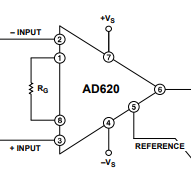
\includegraphics[width=0.4\textwidth]{pictures/hardware/Analog_Interface_board/AD620A.PNG}
	\caption{Instrumentation amplifier AD620A}
	\label{fig:AD620A}
\end{figure} 

The input reference to the \textit{AD620A} has to be very exact. Small differences can cause great inaccuracies in the current measuring. Therefore a voltage reference is used to keep a stable voltage at $0.5V$. The used voltage reference used is a \textit{LM385Z-1.2} in conjunction with a voltage divider of resistors $R1 = 1k\ohm$, $R2 = 1k\ohm$, $R3 = 470\ohm$ yields a constant voltage of

\begin{equation}
	V = V_{ref} \cdot \frac{R1}{R1+R2+R3} = 0.5V
\end{equation}

where 

\begin{equation}
V_{ref} = 1.235V
\end{equation}

A buffer is added to give a low impedance signal to the \textit{AD620A}.

At the input of the instrumentation amplifier a resistor is placed at both the inverting and the non-inverting input to reduce current. Using the \textit{AD620A} is also advantageous for its high CMRR (Common-mode Rejection ratio) that helps with cancelling out noise present on both input pins with the same waveform. It can also use the $\pm15V$ dual supply present on the board.

\subsubsection{Torque pedal measurement}
The output of the torque pedal connects to the same ADC as one of the current channels, hence it also has to be in the range of $0-1V$. The pedal is basically a $7.5k\ohm$ potmeter, so the idea is to parallel it with the lower resistor of a voltage divider to get about $1V$ at full range. Using $V_{ref_3} = 3.3V$ as excitation for the divider and $R1 = R2 = 10K\ohm$, the following equation is true at full throttle: 

\begin{equation}
	V = V_{ref_3} \cdot \frac{R_{pot} \cdot R15}{R_{pot} \cdot R15 + R14} = 0.99V
\end{equation}

When the pedal is not pressed at all, the $0\ohm$ of the potmeter shunts the supply to the ground.

\begin{figure}[H]
\centering
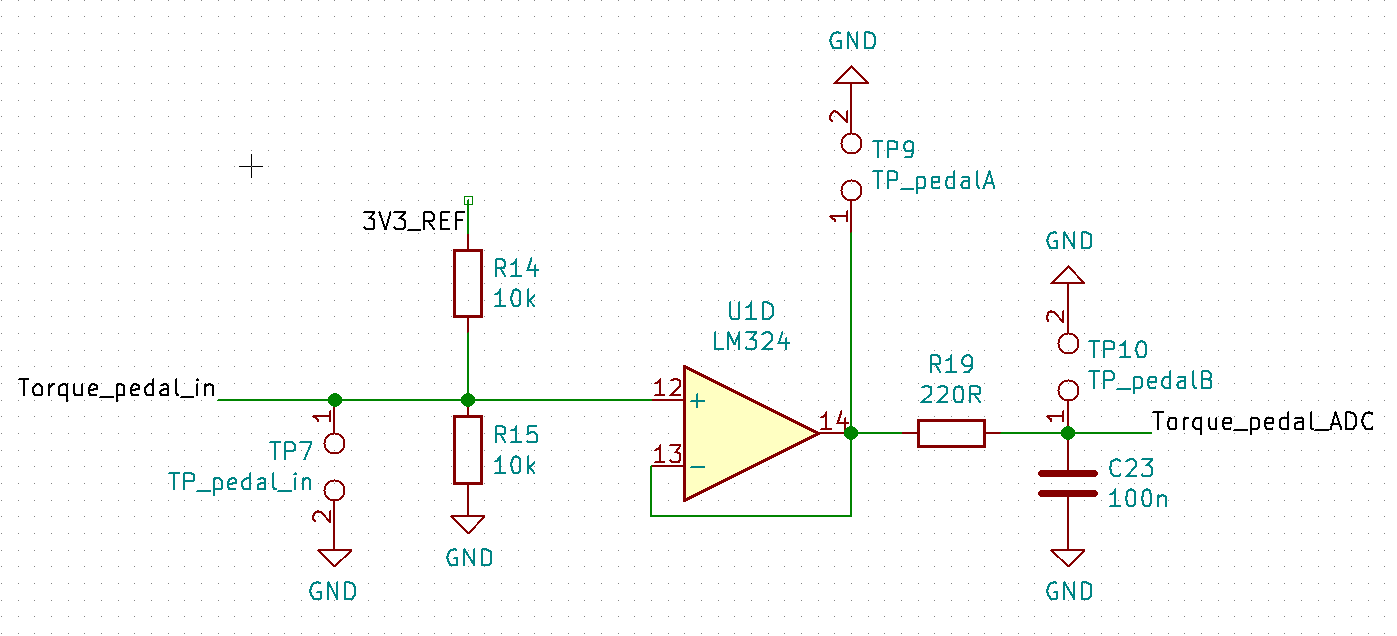
\includegraphics[width=1\linewidth]{pictures/hardware/Analog_Interface_board/torque_pedal_divider.png}
\caption{Torque pedal reading circuit}
\label{fig:torque_pedal_divider}
\end{figure}

For this channel, an opamp in voltage follower configuration is sufficient instead of an instrument amplifier, since no offsetting is required.

\subsection{Power board}
The inverter is divided into two PC boards, one for the high power part, the Power board and one for the driver part, the Driver board. In this section is it described how the Power board for the inverters is designed and what considerations have been made. It will be described what kind of PCB and which components has been used and why. The layout of the inverter power board will also be described and which choices has been made doing that.
\\
The objective is to design a two level three phase inverter to drive the go-carts PMSM motor. This basically consist of six switches and some capacitance on the DC-link. On figure \ref{fig:Sketch_PowerBoard} a simple model of the Power board is shown.

    \begin{figure}[H]
		\centering
		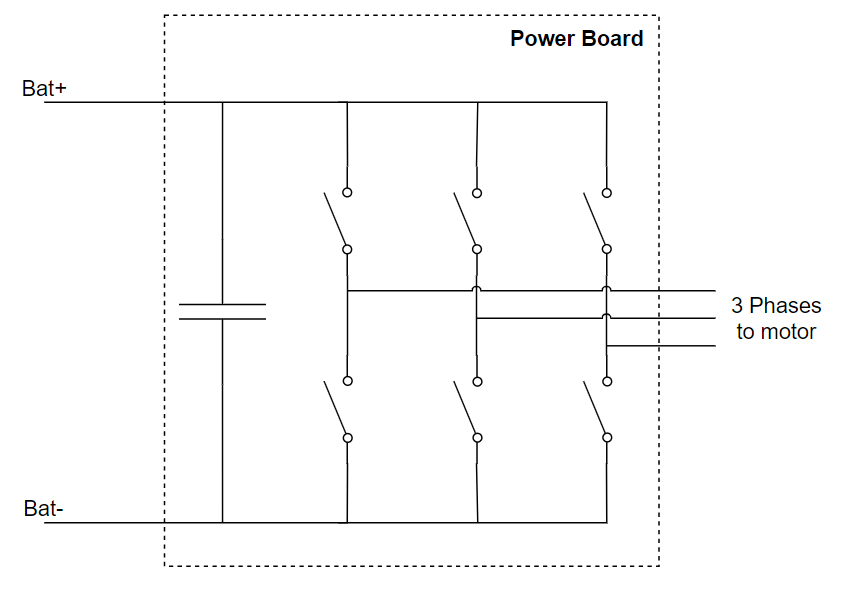
\includegraphics[width=0.7\textwidth]{pictures/hardware/Power_Board/Sketch_of_powerBoard.PNG}
		\caption{Sketch of the Power Board}
		\label{fig:Sketch_PowerBoard}
	\end{figure} 
	
This means that there have to be selected a switch component. The switch component has a great impact on the inverter design, due to that it is a big source of losses in the inverter. It is therefore important to choose a good transistor for switching. Besides the switch component, there has to be selected a type PCB board for the Power board.

\subsubsection{Switching frequency} \label{switching_frequency}
When deciding a switching frequency for the inverters, the rotation frequency of the motor and the thus the frequency of the electrical field.
It is known form the Data sheet of the motor, that the maximum rotation speed of the motor is $5000 rpm$ and it has 8 poles equal to 4 pole pairs. From this the maximum frequency of the electrical field be determined.

\begin{equation}
    f = \frac{v_{rpm} \cdot P}{60}
    \label{eq:max_frequency}
\end{equation}

Where $v_{rpm}$ is the rotational speed in $rpm$ and $P$ is the number of pole pairs in the motor.
From equation \ref{eq:max_frequency} the maximum frequency of the electrical field is $333.3 Hz$.
It is desired to have between 10 and 20 switch periods per period of the electrical field. 20 switch periods per electrical field period results in a switching frequency of $6666 Hz$. It is not necessary to switch faster than the $6666 Hz$, but it is decided to use a switching frequency of $10 kHz$. This is done to make the use of smaller capacitors possible and because already so low frequency it is not a problem to increase it a bit.
It is decided not to increase the switching frequency to more than $10 kHz$ to reducing the switching losses.


\subsubsection{PCB selection}   \label{PCB_selection}
Two types of PCB's has been considered, a ordinary multi-layer PCB and a single-layer aluminum PCB. There is of course pros and cons for both options. With the ordinary PCB there is better opportunities for conducting the heat away from the switch components. On the other hand it is not possible to use SMD components, due to the heat can not be transferred away from the components. The SMD components can result in a better and more compact layout. This is due to the SMD components is smaller and is available with multiple source legs, which minimize the common source for the switch components. The Use of SMD components will be possible with the aluminum PCB. Due to that the SMD components have a smaller area and the heat has the transferred through the aluminum PCB, the cooling of the components is a harder task. With the aluminum PCB it is not possible to use through hole components, which can have some cons when it comes to the mounting of the large capacitors for the DC-link. 

 The ordinary PCB has also the benefit, that is has multiple layers. This could make it easier to layout a good power board. On the other hand, due to the budget, it will not be possible to get a PCB with much more than 2 layers anyways, maybe 4 layers. It is of course better than the single layer on the aluminum PCB. It is possible to get the aluminum PCB with two layers, but it will result in a  too high thermal resistance and price.

Based on these considerations it is chosen to use the aluminum PCB, because the benefits of the SMD components is weighted higher than the cons.


\subsubsection{Transistor selection}
Transistors selection is an important aspect in the design of the inverter. This due to that the transistors has great affect on the power loss in the system and thus the heat dissipation which set the limits of the design. Transistor selected is made from a couple of aspects. first of all the needed ratings necessary for the system. The Drain to Source current has to be rated for $300 A$ if no parallel devices is used. It is chosen that it has to have a rated Drain to Source voltage of $100 V$. This is due to the battery in the go-kart has a maximum voltage of $57.6$ plus some safety margin for voltage spikes. The maximum battery voltage is found based on the cell voltage of a $LiFePO_4$: $3.6 V$, multiplied with the number of cells, which is 16. The transistor has to have a fall time of less than $250ns$ and rise time of less than $50ns$. Besides that the transistor has to have a as low as possible on-resistance, to minimize conduction losses, which is very significance when conducting a current of $300A$.

The Transistor with these specifications and the lowest possible Drain-Source on resistance, to a affordable price, was a MOSFET. The MOSFET have the benefit of having a low current needed for turn on, the ability to handle high current needed for the motor and fast enough for the switching frequency. Since price is everything, when it comes to choice of components, then some sort of compromise will be made \\

The MOSFET chosen is an Infineon "IPB017N10N5". Some of the important specifications is listed in the table below.
\begin{table} [H]
\centering
 \begin{tabular}{|c|c|c|} 
 \hline
 \textbf{Parameters} & \textbf{Value} & \textbf{Unit} \\
 \hline
 \textbf{$V_{DS}$} & $100$ & $V$ \\  
 \hline
 \textbf{$R_{DS-ON}$} & $1.7$ & $m\Omega$ \\
 \hline
 \textbf{$I_D$} & $273$ & $A$ \\
 \hline
 \textbf{$Q_G\ (0-10V)$} & $168$ & $nC$ \\
 \hline
 \textbf{$Q_{GD}$} & $34$ & $nC$ \\
 \hline
 \textbf{$Q_{GS}$} & $53$ & $nC$ \\
 \hline
 \textbf{$Q_{sw}$} & $51$ & $nC$ \\
 \hline
 Rise time & $23$ & $ns$ \\
 \hline
 Fall time & $27$ & $ns$ \\
 \hline
\end{tabular}
\caption{Transistor parameters taken from the "IPB017N10N5" datasheet}
\end{table}

When looking at the parameters, a couple of things need to be considered. From the top it can be seen that the Drain-Source voltage is $100 V$, so it is able to handle the kart's battery voltage. Next the  [$I_D$] is not $300 A$ or above, which leads to a design choice of having two or more in parallel. Having more transistors in parallel has the benefit of splits the current up between them, lowering the conduction power loss. Having lower power loss decreases the amount of heat generated, which leads to less risk of overheating. The gate charge is the amount of charge that needs to be delivered to the gate from the driver, in order to turn the transistor on. This parameter needs to be as low as possible same as the Drain-Source resistance, but normally with a low resistance comes higher gate charge and vise versa. In this case is it more important that the Drain-Source on resistance is low rather than the Gate charge is low. This is the case because speed of the turning on and off of the MOSFET is reduced anyway. Besides that the increased driver power losses will not be as significant compared to the increased power losses in a MOSFET with higher Drain-Source on resistance.\\ 


\subsubsection{Power and heat dissipation in the transistors}
There are two types of power losses in the transistors. One is conduction losses, which is caused by the intern resistance in MOSFET between the Drain and the Source, when the MOSFET is conducting. The other one is switching losses, which is caused then the MOSFETs is turning on and off. Based on the power loss calculations the expected heat increase of the MOSFETs can be estimated, which will be used to decide how many MOSFETs in parallel is needed.

\paragraph{Conduction power loss}
When a MOSFET is conducting there will be a power dissipation due to the intern Drain-Source on resistance in the MOSFET. Thus the conduction power loss in the MOSFETs is calculated in the same way as the power loss in a resistor. Equation \ref{eq:ConductionLossMOSFET} describes the conduction power loss for one MOSFET, $P_{con/MOSFET}$.

    \begin{equation}
        P_{con/MOSFET} = \bigg( \frac{I}{N \cdot 2} \bigg) ^2 \cdot R_{DS-ON}
        \label{eq:ConductionLossMOSFET}
    \end{equation}

$I$ is the peak current, $N$ is the number of transistors in parallel per switch, and $R_{DS-ON}$ is the Drain-Source on resistance of the MOSFET.
The peak current is divided by the number of transistors in parallel, to get the current in one MOSFET. Because the current is sinusoidal and the average duty cycle of the PWM over a period is $50 \% $, it is also divided by two to get the current one transistor is conducting.

To calculate the conduction power loss for all the transistors, it is then multiplied with the number of parallel MOSFETs per switch, two for taking both the high and low side into account, and the number of legs in the inverter, which is three.

    \begin{equation}
        P_{con} = \bigg( \frac{I}{N \cdot \sqrt{2}} \bigg) ^2 \cdot R_{DS-ON} \cdot N \cdot 2 \cdot 3
        \label{eq:ConductionLossTot}
    \end{equation}

On figure \ref{fig:ConductionLoss} the relationship between conduction power loss per MOSFET, equation \ref{eq:ConductionLossMOSFET}, and for all the MOSFETs, equation \ref{eq:ConductionLossTot}, is plotted as a function of the number of MOSFETs in parallel. 

    \begin{figure}[H]
		\centering
		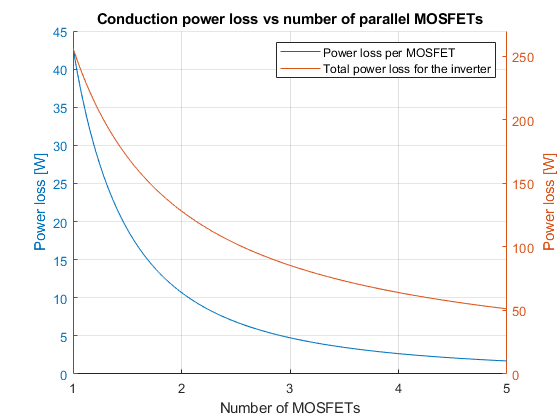
\includegraphics[width=0.8\textwidth]{pictures/hardware/Power_Board/Conduction_loss.png}
		\caption{Conduction power loss versus the number of parallel transistors in parallel per switch}
		\label{fig:ConductionLoss}
	\end{figure} 

For figure \ref{fig:ConductionLoss} the peak current, $I$, is set to $300 A$, and the Drain-Source on resistance, $R_{DSon}$, is set to ${1.9 m \Omega}$, which is value at $80 \degree C$. \todo{ref to data sheet}

On figure \ref{fig:ConductionLoss} it can be seen that the more MOSFETs there are placed in parallel per switch, the conduction power losses reduces exponentially, for both each MOSFET and for the hole inverter.

\paragraph{Switching power loss}
The other cause of power loss in the MOSFETs is the switching power loss. The switching power losses is caused by the period, when switching, where both the voltage over and the current through the MOSFET is not zero. This is called hard switching. Soft switching is when the MOSFET switching on or off without the voltage and current overlaps. This will not cost any power loss. This is illustrated on figure \ref{fig:HardSoftSwitch}.

    \begin{figure}[H]
		\centering
		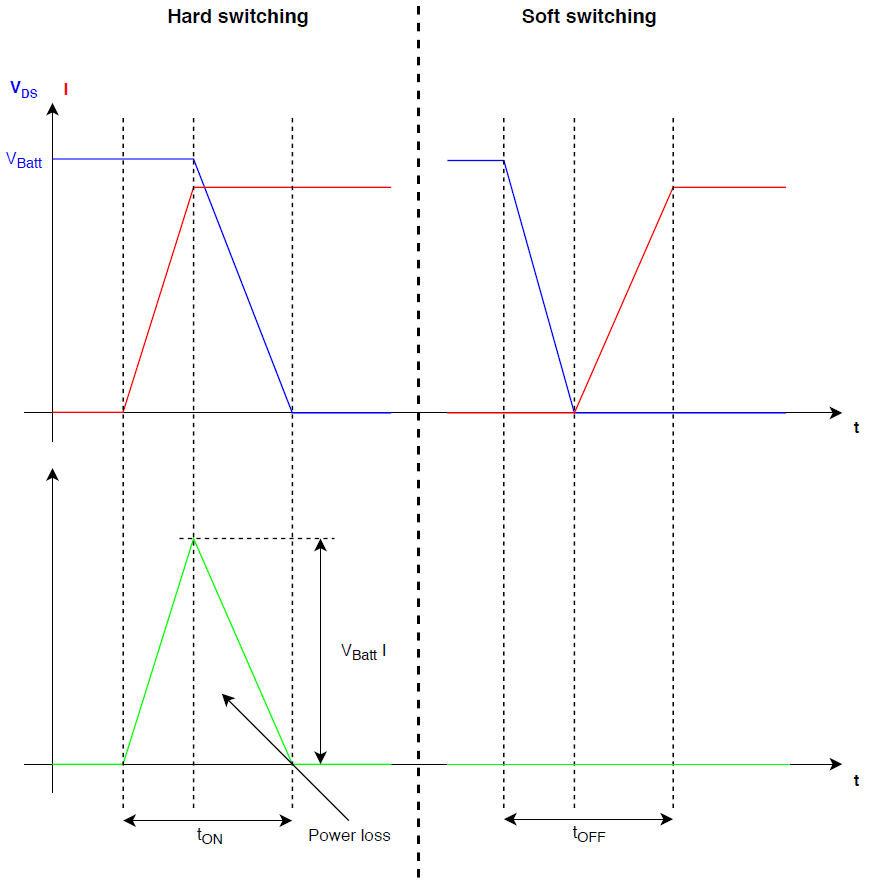
\includegraphics[width=0.8\textwidth]{pictures/hardware/Power_Board/Hard_soft_switching.PNG}
		\caption{Illustration of hard and soft switching of MOSFET}
		\label{fig:HardSoftSwitch}
	\end{figure} 

When running the motor, the motor current has a positive and a negative half cycle. During the positive half period the current going into the motor, and in the negative half period the current going from the motor into the inverter. In the positive half period the low-side switch gets soft turned on and the high-side switch gets hard turned on. Opposite in the negative half period the low-side switch is hard turned on and the high-side switch is soft turned on. This means One transistor will only hard switch $50 \%$ of the time.

The switching power is calculated as the area under the green line on figure \ref{fig:HardSoftSwitch} multiplied with the switching frequency. This is multiplied with a half because the switches is only hard switched $50 \%$ of the time, and therefore the Power loss is the half. 

    \begin{equation}
        P_{sw/MOSFET} = 0.5 \cdot 0.5 \cdot V_{batt} \cdot \frac{I}{N} \cdot (t_{on}+t_{off}) \cdot f_{s}
        \label{eq:sw_loss_MOSFET}
    \end{equation}

Where $V_{batt}$ is the battery voltage, $t_{on}$ is the turn on time, $t_{off}$ is the torn off time, and $f_{s}$ is the switching frequency of the transistors.
Equation \ref{eq:sw_loss_MOSFET} is the switching power loss per MOSFET. To get the switching power loss for all of the MOSFETs in the inverter, this has to be multiplied with the number of parallel MOSFETs, two to take both the high- and low-side into to account, and the number of phases, which is three.

    \begin{equation}
        P_{sw} = 0.5 \cdot 0.5 \cdot V_{batt} \cdot \frac{I}{N} \cdot (t_{on}+t_{off}) \cdot f_{sw} \cdot N \cdot 2 \cdot 3
        \label{eq:sw_loss}
    \end{equation}
    
From this equation, a curve of the switching power loss in one MOSFET and in all the MOSFETs versus the number of the parallel MOSFETs, is made.

    \begin{figure}[H]
		\centering
		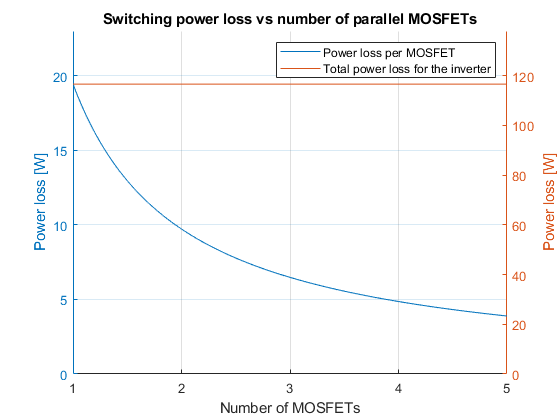
\includegraphics[width=0.8\textwidth]{pictures/hardware/Power_Board/Switch_loss.png}
		\caption{Conduction power loss versus the number of parallel transistors in parallel per switch}
		\label{fig:sw_loss}
	\end{figure}
	
Again is the peak current, $I$, is set to $300 A$. The battery voltage, $V_{batt}$, is set to $57.6 V$ and the switching frequency is set to the chosen frequency: $10 kHz$. The turn on time, $t_{on}$, and the turn off time, $t_{off}$, is calculated with the following equations.

    \begin{equation}
        t_{on} = \frac{Q_{sw}}{I_{GSource}}
    \end{equation}
    
    \begin{equation}
        t_{off} = \frac{Q_{sw}}{I_{GSink}}
    \end{equation}
    
Where $Q_{sw}$ is the switching charge of the MOSFET, which is stated in the Data sheet.\cite{mosfet}
$I_{GSource}$ and $I_{GSink}$ is respectively the current the driver deliverers to the Gate of the MOSFET when turning the MOSFET on and off. These are calculated in section \ref{sec:DriverDesign}. The turn on and off end up being $75 ns$ and $375 ns$, which could be faster, but is chosen to be limited to this. This is due to reducing high-frequency ringing when switching the MOSFETs. This results in a higher switching power loss, but because the switching loss does not have that big of an impact on the total power loss, due to the low switching frequency, it is not considered a problem.

On figure \ref{fig:sw_loss} it can be seen that the switching power loss of each MOSFET is reduced with number of parallel MOSFETs, but the over all power loss of the inverter is the same independent of the number of parallel MOSFETs.

\paragraph{Heat dissipation}
Now when the conduction power loss and switching power loss is determined compared to the number of MOSFETs, the total power losses is known. From the total power loss in the transistors the heat dissipation, depending on the number of MOSFETs, can be determined.

When determine the heat dissipation of the inverter, all the thermal resistances between the junction of the MOSFET and the ambient has to be specified.
First of all there is the internal junction to case resistance for the MOSFET.
When using the aluminum PCB with the SMD components, the heat has to be transferred through the PCB. This means this adds an extra thermal resistance to the system. The aluminum PCB is divided into three parts, the copper layer, a dielecrical layer for isolating the copper from the aluminum, and the aluminum layer.
Then there is a thin layer of thermal paste to connect the PCB to the heat sink. And the last resistance before the ambient is the heat sink. This is illustrated on figure \ref{fig:thermal_overview}.

    \begin{figure}[H]
		\centering
		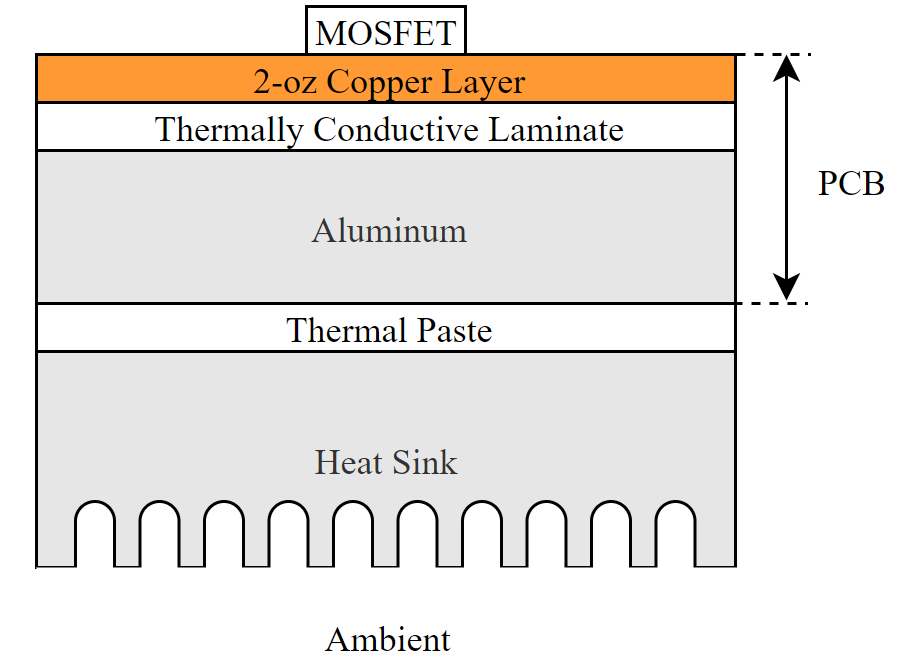
\includegraphics[width=0.6\textwidth]{pictures/hardware/Power_Board/Thermal_overview.png}
		\caption{Overview of the thermal resistances between the junction of the MOSFET and ambient}
		\label{fig:thermal_overview}
	\end{figure}
	
The thermal resistance from the junction to the case of the MOSFET is stated to be $0.4 K/W$ in the data sheet for the MOSFET.\cite{mosfet}
The thermal resistance of the copper layer, is calculated from equation \ref{Rthermal}

    \begin{equation}
        R_{thermal} = \frac{t_{layer}}{A_{MOSFET} \cdot k_{material}} 
        \label{Rthermal}
    \end{equation}
    
Where $t_{layer}$ is the thickness of the layer in $m$, $A_{MOSFET}$ is the surface area of the MOSFET in $m^2$, and $k_{material}$ is the thermal conduction constant for the layer material in $\frac{W}{m \cdot K}$.

The thickness of the copper layer is known to be $1 oz/foot^2$ from 'pcbway.com', which is converted to $34 \cdot 10^{-6} m$ from the density of copper. The area of the surface area of the MOSFET is found in the data sheet to be $63 \cdot 10^{-6} m^2$.\cite{mosfet} The area of the MOSFET is used all the way down to the heat sink, because it is assumed that the heat will go straight through the PCB and the paste. This is most likely not the case but that will be the worst case.
The thermal conduction constant of copper is $401 \frac{W}{m \cdot K}$.\cite{toolbox}

The thermal resistance of the dielectrical layer is calculated based on the same equation as \ref{Rthermal}.

Where the thickness of the dielectrical layer is $100 \mu m$, which is stated by the manufactore, pcbway.com. The thermal conduction constant is chosen to be $1 \frac{W}{m \cdot K}$. The manufacture offers also the aluminum PCB with a dielectrical layer with a thermal conduction constant of $2 \frac{W}{m \cdot K}$, but due to price this was not chosen.

Equation \ref{Rthermal} is used again for calculating the thermal resistance of the aluminum layer of the PCB.
Where the he thickness of the aluminum layer is the chosen PCB thickness of $0.8 mm$ minus the thickness of the two other layers. The thickness of $0.8 mm$ is chosen because that is the thinnest option without getting the PCB more expensive. The thermal conduction constant for aluminum is $236 \frac{W}{m \cdot K}$.\cite{toolbox}

The thermal resistance for the total PCB is then:

    \begin{equation}
        R_{PCB} = R_{copper} + R_{del} + R_{alu}
        \label{RPCB}
    \end{equation}

Where $R_{copper}$ is the thermal resistance of the copper layer, $R_{del}$ is the thermal resistance of the dielectrical layer, and $R_{alu}$ is the thermal resistance of the aluminum layer.

To calculate the thermal resistance of the thermal paste, equation \ref{Rthermal} is used as well. The thickness of the paste is estimated to be $0.1 mm$ and the thermal conduction constant of the paste is set to $3 \frac{W}{m \cdot K}$. This based on values for different thermal paste, and then a value close to the average of them was chosen.

This results in, that the total temperature difference from the thermal paste to the MOSFET junction can be calculated with equation \ref{eq:tempMOSFET}.

    \begin{equation}
        T_{JP} = P_{loss/MOSFET} \cdot (R_{JC} + R_{PCB})
        \label{eq:tempMOSFET}
    \end{equation}
    
Where $R_{JC}$ is the internal junction to case thermal resistance and $P_{loss}$ is the total power loss for one MOSFET. 

To calculate the temperature difference over the heat sink, the average power loss is used instead of the maximum power loss. This is done because the heat sink has a higher thermal capacitance, and therefore is less reactive to changes in temperature. The average power loss is calculated in the same way as the maximum power loss, but instead of using the maximum current a average current is estimated. The average current is estimated to $75 A$.
From this the temperature difference over the heat sink is calculated, with equation \ref{Theatsink} 

    \begin{equation}
        T_{HA} = P_{Avg} \cdot R_{HA}
        \label{Theatsink}
    \end{equation}

The $P_{Avg}$ is the average power loss for all the MOSFETs and $R_{HA}$ is the thermal resistance of the heat sink. 


% \subsubsection{Design}

The $V_{DS}$ fall time (the MOSFET switch-in time) is slowed down to $\approx 250ns$ and the rise time (switch-off) is $\approx 50ns$. The required resistor values can be calculated using Equation \ref{eq:i_Gsink_per_fet_1} through Equation !!!. \\

To get the resistor values, first, the sink current must be calculated for the required switch-off time for the individual MOSFETs.

    \begin{equation}
        i_{Gsink/FET} = \bigg( \frac{Q_{GD}}{t_{sw{\_}off}} \bigg)
        \label{eq:i_Gsink_per_fet_1}
    \end{equation}
    
    where
    
    \begin{itemize}
        \item $i_{Gsink/FET}$ is the required switch-off current
        \item $Q_{GD}$ is the gate-drain charge of the MOSFET
        \item $t_{sw{\_}off}$ is the desired switch-off time
    \end{itemize}
    
    \begin{equation}
        i_{Gsink/FET} = \bigg( \frac{V_{Miller}}{R_{G{\_}FET} + R_{G{\_}FET{\_}int}} \bigg)
        \label{eq:i_Gsink_per_fet_2}
    \end{equation} \\
    
    Rearranging Equation \ref{eq:i_Gsink_per_fet_2} yields the following:
    
    \begin{equation}
        R_{G{\_}FET} = \bigg( \frac{V_{Miller}}{i_{Gsink/FET}} - R_{G{\_}FET{\_}int} \bigg)
        \label{eq:i_Gsink_per_fet_2}
    \end{equation}
    
    where
    
    \begin{itemize}
        \item $R_{G{\_}FET}$ is the resistor for the individual MOSFETs
        \item $V_{Miller}$ is the Miller-plateau of the MOSFET
        \item $R_{G{\_}FET{\_}int}$ is the internal gate-source resistance of the MOSFET
    \end{itemize}
    
    Now the common resistance can be calculated:
    
    \begin{equation}
        i_{Gsource/FET} = \frac{\frac{V_G - V_{Miller}}{R_{pullup} + R_G}}{N}
        \label{eq:i_Gsoursce_per_fet_1}
    \end{equation}
    
    where
    
        \begin{equation}
        i_{Gsource/FET} = \frac{\frac{V_G - V_{Miller}}{R_{pullup} + R_G}}{N}
        \label{eq:i_Gsoursce_per_fet_1}
    \end{equation}
    
    Rearranging Equation \ref{eq:i_Gsoursce_per_fet_1} yields the following:
    
    \begin{equation}
        i_{Gsource/FET} = \frac{\frac{V_G - V_{Miller}}{R_{pullup} + R_G}}{N}
        \label{eq:i_Gsoursce_per_fet_1}
    \end{equation}
% \subsubsection{Implementation}

\subsection{Driver board}
This section describes the theoretical background, the design considerations taken and the implementation of the driver circuit and the PCB.
\subsubsection{Analysis}
The gate driver selected for this design is the SI8261BAC-C-IS\cite{Si8261} from Silicon Labs. It is driven by the $3.3V$ output of the Zybo while providing an output of $12V$, constrained by the attached $12V$ floating supply Cosel MGS1R54812\cite{MGS1R5}. A floating supply is required for the high-side to be able to take on a potential independent of the power ground when its drain and source potential is constrained by the load and the battery voltage. The gate driver's ground floats along with the source potential of the FET so it is always able to provide a voltage of $12V$ between the gate and the source. The advantage of having an isolated supply for the low-side as well is better noise tolerance - the FETs reference level is made somewhat independent of the ripple current on the power ground from all the loads. The high-side floating supply also has the advantage over a bootstrap capacitor of not requiring  part of an output cycle to be used for charging the capacitor. This way more power can be used to propel the gokart.

\begin{figure}[H]
	\centering
	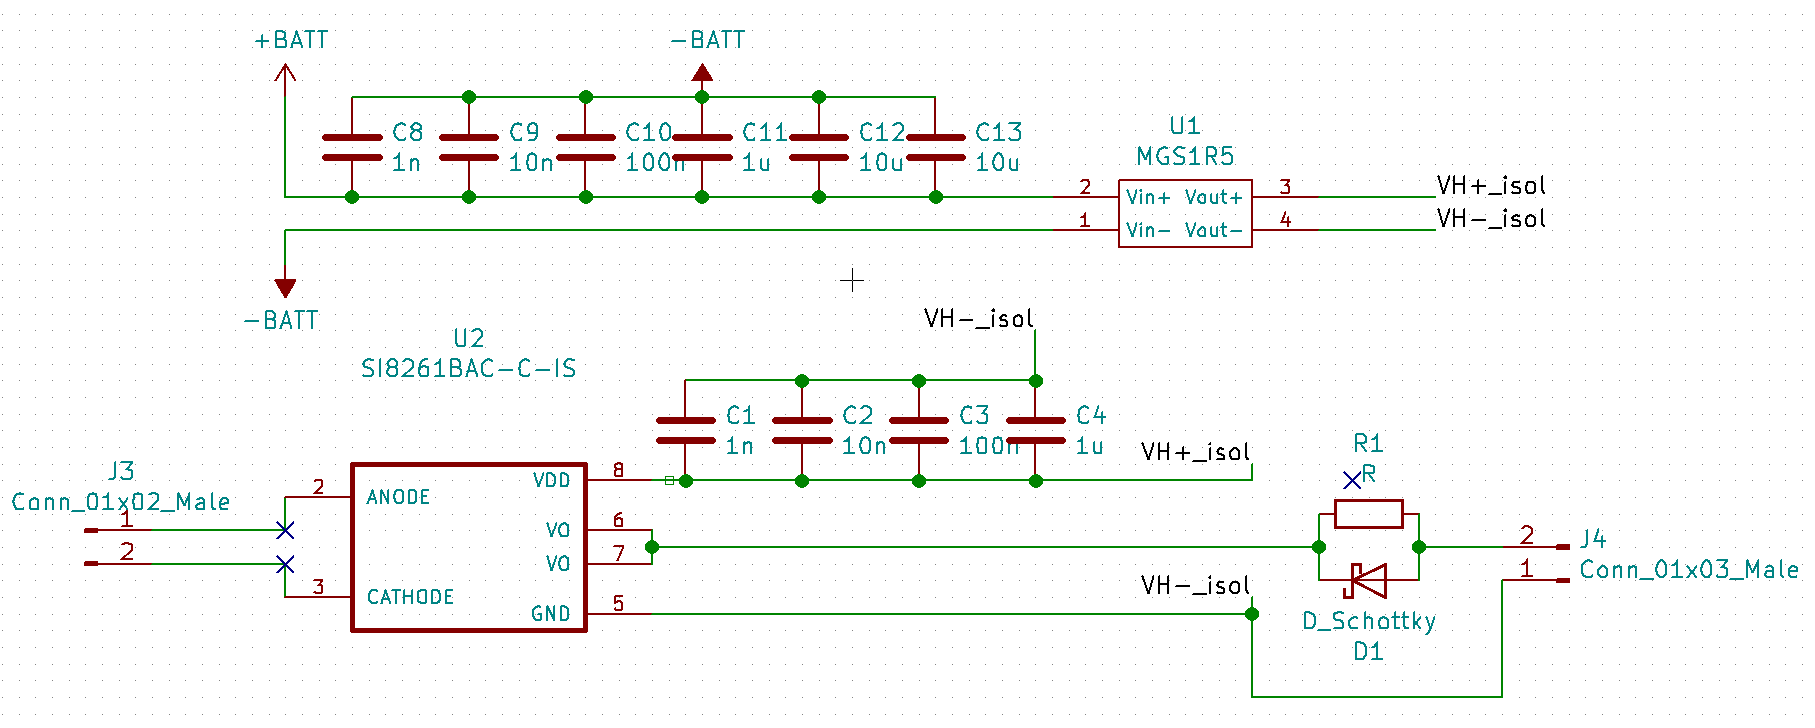
\includegraphics[width=0.6\linewidth]{pictures/hardware/Driver_Board/driver_circuit.png}
	\caption{One leg of one phase of the driver circuit}
	\label{fig:driver_circuit}
\end{figure}

 Figure \ref{fig:driver_circuit} shows the driver of one leg of one phase. Separate drivers were chosen for the separate legs of each phase to reduce the thermal stress of the individual IC-s. The low-side and the high-side driver circuit is identical. \\

A series of capacitors is attached both to the input and output of the floating supply. The smaller ones are meant to serve as high-frequency decouplers while the $10$$\mu$$F$  ones are the bulk capacitors to prevent droop on the $12V_{DC}$ rail. This helps with countering the noise-emitting effects of the long wires and quick transients from the battery when load changes rapidly. \\

The turnon and turnoff times were chosen to be around the slower end of the available range to make the circuit less prone to overshoot and ringing caused by the parasitic inductances and capacitances inherently present in the layout. The analysis of deciding the switching frequency is detailed in section \ref{switching_frequency}. \\

In Figure \ref{fig:CSI_current} and Figure \ref{fig:skew_current} taken from TIDA-00364\cite{TIDA-00364} reference design by TI, the use of split gate resistors can be seen. These consist of R2, which is common to all the parallel MOSFETs, and R20 through 24, which are individual to each MOSFET . R2 helps to easily change the turnon gate current of all the parallel FETs by changing a single resistor instead of changing each of the individual resistors. R20 through R24 help in suppressing the circulating current between the gate of the MOSFETs, which may cause gate voltage ringing. To describe the mechanism, consider only two FETs in parallel as shown in Figure \ref{fig:CSI_current} . Due to the layout, the parasitic common source inductance (CSI) of all the FETs will not be equal. If both the FETs are turned on the same instant and if the di/dt of the drain currents are equal, the voltage across CSI of both FETs (VLs1 and VLs2) will not be equal. This drives a circulating current as shown in Figure \ref{fig:skew_current} . Another possibility is if there is a skew in the $V_{DS}$ rise and fall time of the parallel FETs, circulating current can flow through the $C_{GD}$ as shown in Figure \ref{fig:skew_current} and cause unwanted behavior. Using individual gate resistors help to suppress the circulating current and help damp unwanted ringing effects. Due to a misunderstanding, we failed to place split resistors, only one is placed at the output of the driver IC, parallel to a diode meant to provide quicker turn-off times. In the upcoming sections the case of the split resistors will be further examined, as it was the original plan.

\begin{figure}[H]
	\centering
	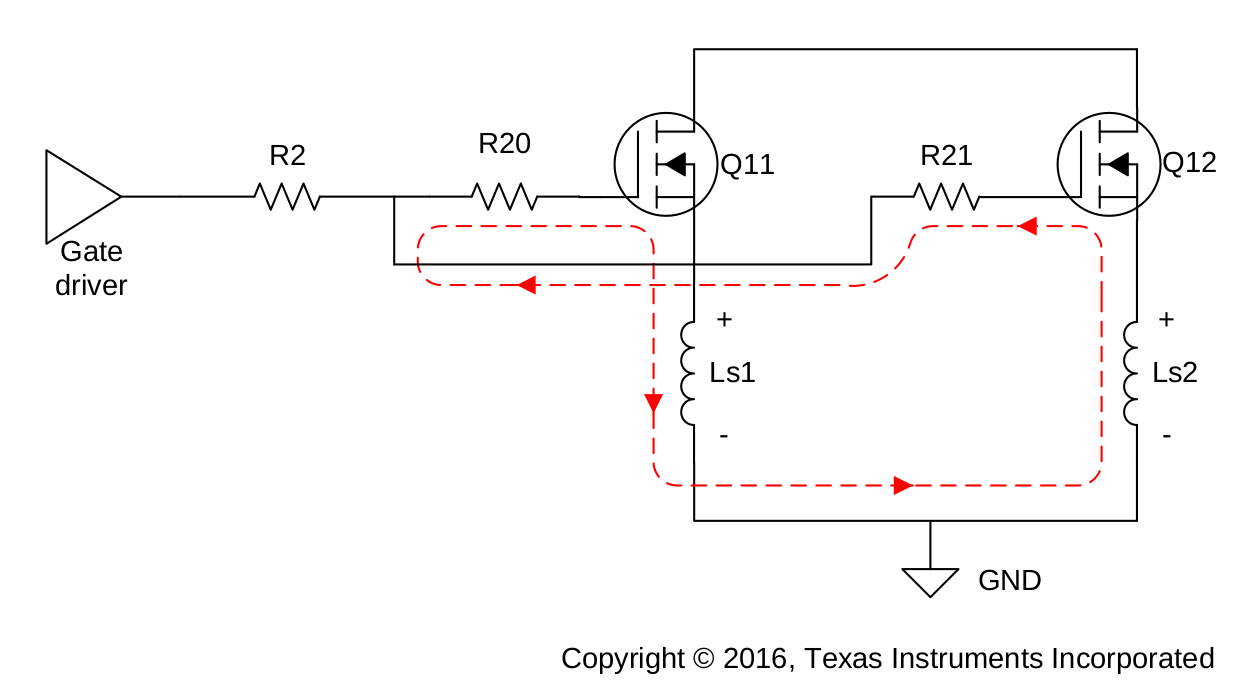
\includegraphics[width=0.6\linewidth]{pictures/hardware/Driver_Board/CSI.png}
	\caption{Gate circulating current due to CSI}
	\label{fig:CSI_current}
\end{figure}

\begin{figure}[H]
	\centering
	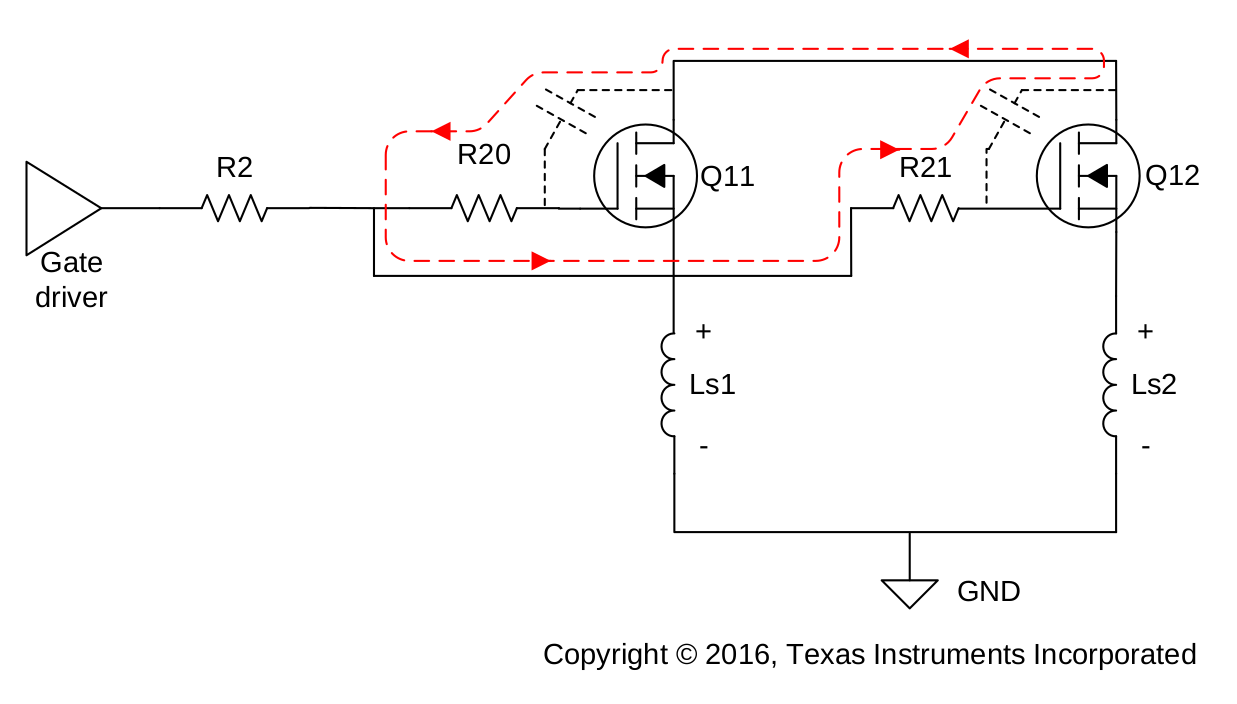
\includegraphics[width=0.6\linewidth]{pictures/hardware/Driver_Board/skew.png}
	\caption{Gate circulating current due to skew}
	\label{fig:skew_current}
\end{figure}
\subsubsection{Design}

The $V_{DS}$ fall time (the MOSFET switch-in time) is slowed down to $\approx 250ns$ and the rise time (switch-off) is $\approx 50ns$. The required resistor values can be calculated using Equation \ref{eq:i_Gsink_per_fet_1} through Equation !!!. \\

To get the resistor values, first, the sink current must be calculated for the required switch-off time for the individual MOSFETs.

    \begin{equation}
        i_{Gsink/FET} = \bigg( \frac{Q_{GD}}{t_{sw{\_}off}} \bigg)
        \label{eq:i_Gsink_per_fet_1}
    \end{equation}
    
    where
    
    \begin{itemize}
        \item $i_{Gsink/FET}$ is the required switch-off current
        \item $Q_{GD}$ is the gate-drain charge of the MOSFET
        \item $t_{sw{\_}off}$ is the desired switch-off time
    \end{itemize}
    
    \begin{equation}
        i_{Gsink/FET} = \bigg( \frac{V_{Miller}}{R_{G{\_}FET} + R_{G{\_}FET{\_}int}} \bigg)
        \label{eq:i_Gsink_per_fet_2}
    \end{equation} \\
    
    Rearranging Equation \ref{eq:i_Gsink_per_fet_2} yields the following:
    
    \begin{equation}
        R_{G{\_}FET} = \bigg( \frac{V_{Miller}}{i_{Gsink/FET}} - R_{G{\_}FET{\_}int} \bigg)
        \label{eq:i_Gsink_per_fet_2}
    \end{equation}
    
    where
    
    \begin{itemize}
        \item $R_{G{\_}FET}$ is the resistor for the individual MOSFETs
        \item $V_{Miller}$ is the Miller-plateau of the MOSFET
        \item $R_{G{\_}FET{\_}int}$ is the internal gate-source resistance of the MOSFET
    \end{itemize}
    
    Now the common resistance can be calculated:
    
    \begin{equation}
        i_{Gsource/FET} = \frac{\frac{V_G - V_{Miller}}{R_{pullup} + R_G}}{N}
        \label{eq:i_Gsoursce_per_fet_1}
    \end{equation}
    
    where
    
        \begin{equation}
        i_{Gsource/FET} = \frac{\frac{V_G - V_{Miller}}{R_{pullup} + R_G}}{N}
        \label{eq:i_Gsoursce_per_fet_1}
    \end{equation}
    
    Rearranging Equation \ref{eq:i_Gsoursce_per_fet_1} yields the following:
    
    \begin{equation}
        i_{Gsource/FET} = \frac{\frac{V_G - V_{Miller}}{R_{pullup} + R_G}}{N}
        \label{eq:i_Gsoursce_per_fet_1}
    \end{equation}

\subsection{Power and Driver board layout}
\subsubsection{Overview}

The proper PCB layout of the driver board is just as essential as that of the power board. To keep the price of the PCBs down, both the power and the driver board has to be kept under $100mm x 100mm$. The layer number of the boards is also a pricey concern. Read more on PCB selection in Section \ref{PCB_selection}. The driver board was designed on 2-layer FR4 1 oz. material. \\

The power board was first laid out to get a precise and optimal placement of the critical components, power rails, outputs and interboard connectors. After that came defining the contour of the driver board, precise placement of interboard connectors and crude placement of components. It is vital for all signals to have their firm ground plane under them to act as reference. That is why the bottom side of the driver board was partitioned according to the components on the top side to have their respective ground planes. The surface of the cooper fills were reduced as much as possible to counter capacitive noise propagation. Supply-ground decoupling capacitors were placed as close to their supported components as possible. 0805 and 1206 size code footprints were placed to have more possibilities for modification or rework if need be. A coutout over the power rails provides space for the electrolitic capacitors attached to the busbar. For approximate mechanical construction, see Figure \ref{fig:mech_top} and Figure \ref{fig:mech_persp}.

\begin{figure}[H]
	\centering
	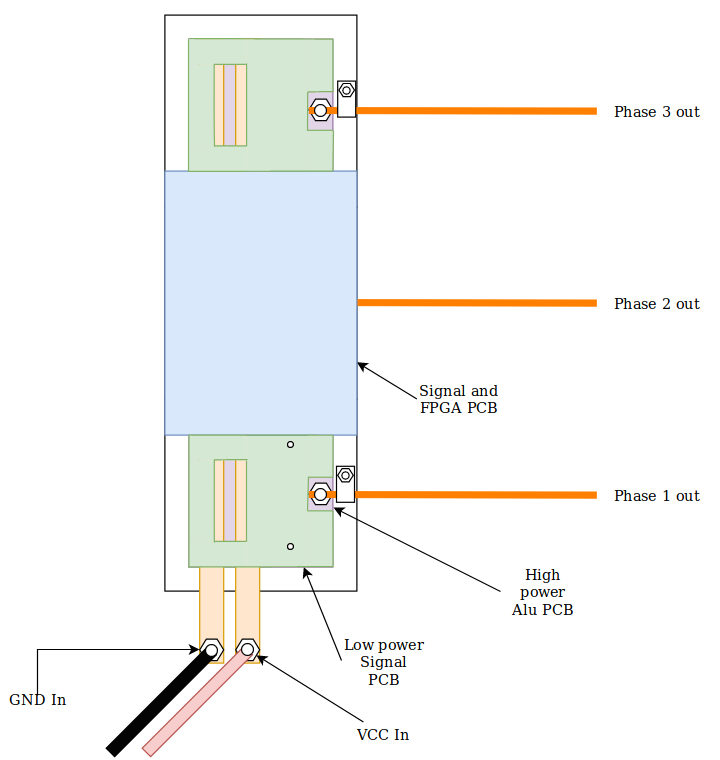
\includegraphics[width=1\textwidth]{pictures/hardware/Power_Board/mechanical_top_new.png}
	\caption{Top view of mechanical construction}
	\label{fig:mech_top}
\end{figure}

\begin{figure}[H]
	\centering
	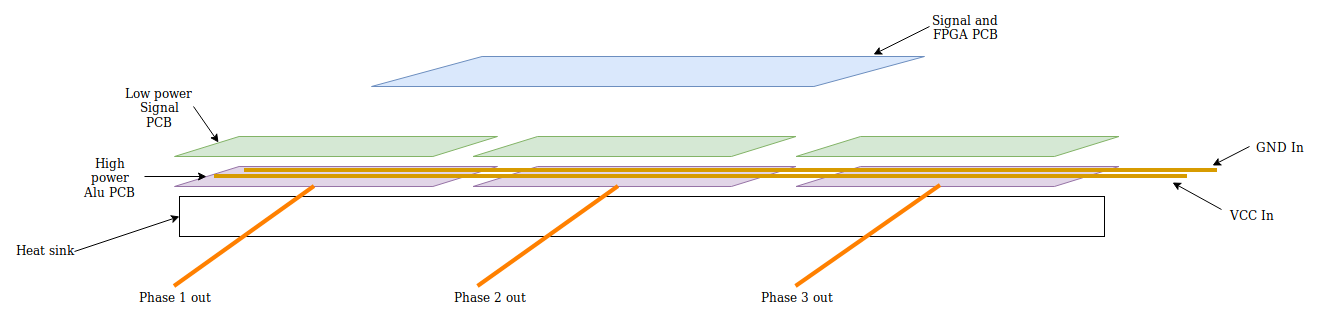
\includegraphics[width=1\textwidth]{pictures/hardware/Power_Board/mechanical_persp_new.png}
	\caption{Perspective view of mechanical construction}
	\label{fig:mech_persp}
\end{figure}

\subsubsection{Power board}

Individual PCBs of $100mm x 65mm$ were chosen for each phase. This way they would be within the general size constraints and fit the $100mm x 200mm$ heatsink that we had available. The three boards are interconnected with the power rail busbars. Only the top side of the alu PCB has a copper layer. This is partitioned into 3 regions. Te first is the battery positive VCC, it is connected to the drain of the high-side MOSFETs. The common region is the output, it gives place to the high-current screw terminal. The source of the low-side FETs is connected to the battery negative GND. To provide the best supply-ground capacitive decoupling and keep the circuit highlighted in \ref{} as short as possible, capacitors are placed along the border of the VCC and GND planes. Electrolitic capacitors sit attached to the busbars. It is important to have as high capacitance ones as possible while keeping the ESR (equivalent series resistance) and stray inductance

\subsubsection{Driver board}